\documentclass[xcolor=pdftex,dvipsnames,table]{beamer}
\usepackage[utf8]{inputenc}
\usepackage[misc]{ifsym}
\usepackage{textpos,tikz,calc,wasysym,xmpmulti}
%% \usepackage{floatrow, pgfplots, enumitem, mathtools, tikz-uml, amsmath, bm}

%% \usetikzlibrary{positioning, shapes}

% \usepackage{beamerthemesplit}
\usetheme{Copenhagen}
% \usecolortheme{structure}
\usefonttheme{professionalfonts}
\setbeamercolor{structure}{fg=black}


\title{3D skeleton extraction for the \emph{Humanitude} project}
\author{Krohg, Bård-Kristian}
\date{April 26th, 2018}


\begin{document}
\maketitle


\begin{frame}
  \frametitle{Overview}
  \begin{itemize}
  \item Introduction
  \item Background
  \item Implementation
  \item Future Work
  \end{itemize}
\end{frame}

\begin{frame}
  \frametitle{Introduction}
  
  %% \begin{columns}[c]
  %%   \column{.75\textwidth}
  %%   \begin{itemize}
  %%   \item[] Bård-Kristian Krohg 
  %%   \item[] University of Oslo / Kyushu University
  %%   \item[] Academic advisors:\begin{itemize}
  %%   \item[] Vice Dean, Professor, Kurazume Ryo 
  %%   \item[] Professor, Jim Tørresen
  %%   \end{itemize}
  %%   \item[] \Letter \hspace{.3em} \texttt{baardkrk@student.matnat.uio.no} 
  %%   \item[] Country of Origin: Norway
  %%   \end{itemize}

  %%   \column{.25\textwidth}
  %%   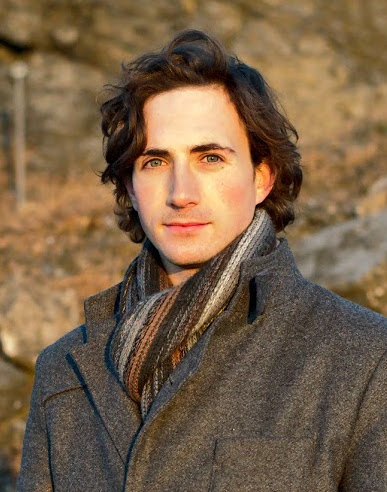
\includegraphics[width=\linewidth]{graphics/selfie.jpg}
  %% \end{columns}


  Theme : 3D skeleton extraction for the \emph{Humanitude} project
  \begin{itemize}
  \item Easy to use \pause
  \item ROS compatible \pause
  \item Markerless \pause
  \item Multi person \pause
  \item Occlusion resistant
  \end{itemize}
\end{frame}

\begin{frame}
  \frametitle{About Humanitude \\ \hspace{20pt}{\small \emph{Background}}}
  \textbf{Humanitude -- Human Attitude}
  
  A way of treating patients developed in France. \pause

  Focuses on the patient being upright, eye contact with the patient, verbal communication and touch. \pause

  Using data gathered from a skilled practitioner of \emph{Humanitude} we hope to provide useful feedback to a student of the method.
  
\end{frame}

\begin{frame}
  \frametitle{3D Keypoints \\ \hspace{20pt}{\small \emph{Background}}}

  We need the pose of both the caregiver and the patient. \pause
  \vspace{10pt}
  
  \textbf{Why 3D?} \pause
\begin{itemize}
\item Interpersonal distance \pause
\item Pose \pause
\item  Setup agnostic 
  \end{itemize}
  
  %% \frametitle{Introduction\\{\small Humanitude Teaching Assistant}}
  %% Using data gathered from a skilled practitioner of \emph{Humanitude} we hope to provide useful feedback to a trainee.\\
  %% \vspace{1em} \pause
  %% \begin{columns}[t]
  %%   \column{.48\textwidth}
  %%   \textbf{Measuring selected features:}
  %%   \begin{itemize}
  %%   \item Posture
  %%   \item Eye contact/motion
  %%   \item Facial expression
  %%   \item Tone of voice
  %%   \item etc.
  %%   \end{itemize} \pause
  %%   \column{.48\textwidth}
  %%   \textbf{Technologies:}
  %%   \begin{itemize}
  %%   \item Multiple RGB-D cameras
  %%   \item OpenPose~\cite{cao2017realtime}
  %%   \item People Localization and Tracking
  %%   \end{itemize}
  %% \end{columns}
\end{frame}

\begin{frame}
  \frametitle{Detecting Humans \\ \hspace{20pt}{\small \emph{Background}}}

    One of the most popular methods : \pause Histogram of Oriented Gradients \pause
    \begin{itemize}
    \item Fast \pause
    \item Well tested \pause
    \item Only location \pause
    \end{itemize}
    \vspace{20pt}
    
    {\Large \textbf{Open Pose}}\pause \\

    Developed at Carnegie Mellon University \pause
    \begin{itemize}
    \item Joint locations (Confidence maps) \pause
    \item Limbs (Part Affinity fields) \pause
    \item Multiple people 
    \end{itemize}
    
\end{frame}

\begin{frame}
  \frametitle{OpenPose Architecture \\ \hspace{20pt}{\small \emph{Background}}}
    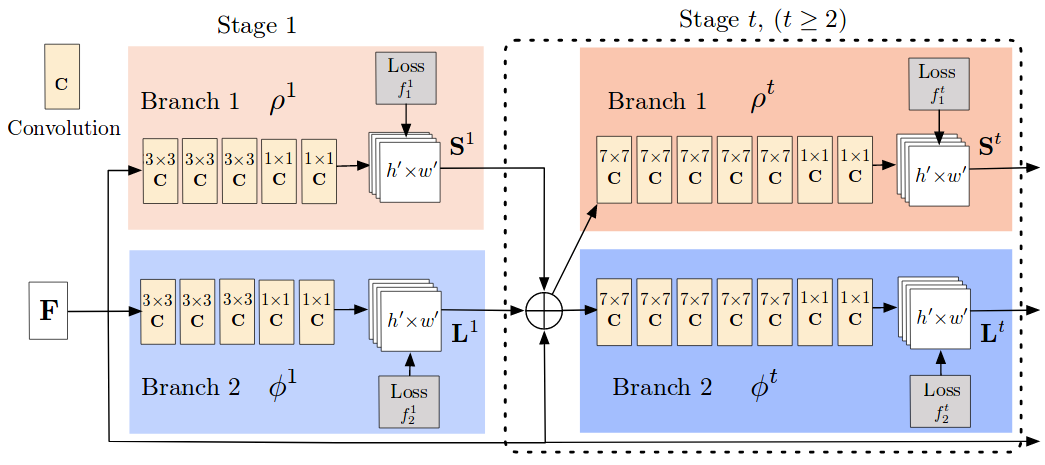
\includegraphics[width=\linewidth]{graphics/openposeArch}
\end{frame}

\begin{frame}
  \frametitle{Implementation}
  \begin{columns}[c]
    \column{.27\textwidth}
    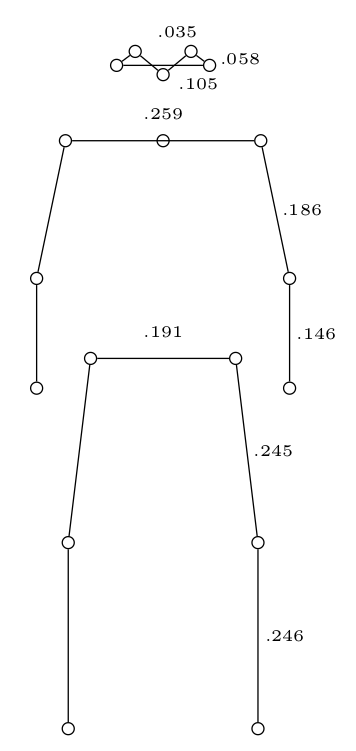
\includegraphics[width=\linewidth]{graphics/constraints}
    \column{.25\textwidth}
    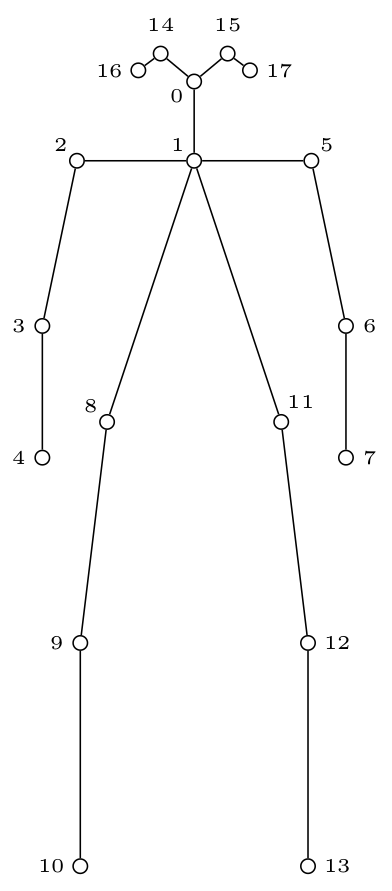
\includegraphics[width=\linewidth]{graphics/keypoints}
  \end{columns}
\end{frame}

\begin{frame}
  \frametitle{Implementation}

  {\large\textbf{ROS Nodes}}

  \begin{itemize}
  \item Kinect subscriber \pause
  \item Info Extractor \pause
  \item Tracker \pause
  \item Renderer \pause
  \end{itemize}
  
\end{frame}


\begin{frame}
    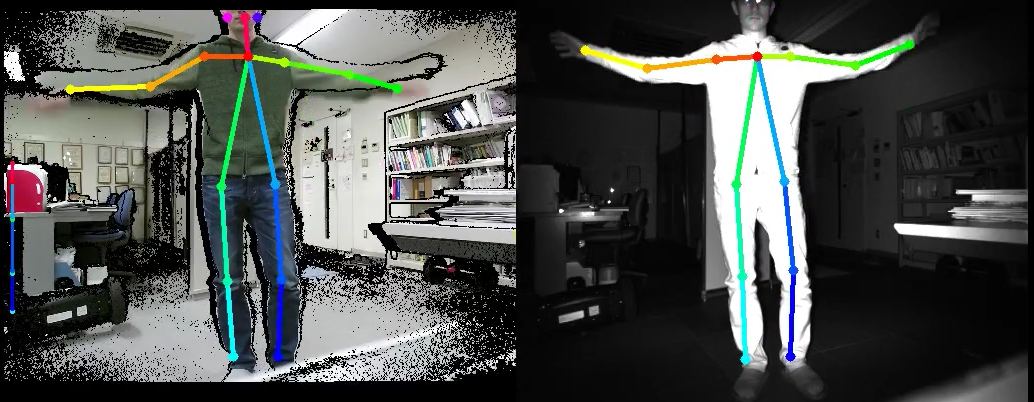
\includegraphics[width=\linewidth]{graphics/rgb_lag}
  \end{frame}

\begin{frame}

  %% \begin{columns}[c]
  %%   \column{.25\textwidth}
    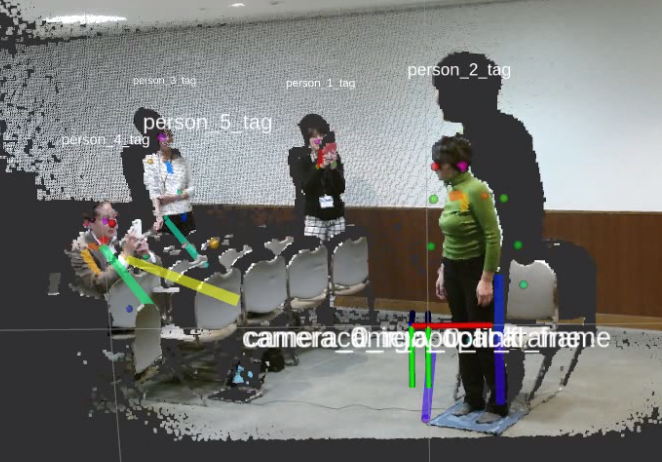
\includegraphics[width=\linewidth]{graphics/tags}
     %% \column{.25\textwidth}

  %% \end{columns}
\end{frame}

%% \begin{frame}
%%   \frametitle{Humanitude}

%%   The Japanese Ministry of Health, Labour and Welfare are evaluating the multimodal comprehensive care methodology called \emph{Humanitude}.\\
%%   \vspace{.7em} \pause
%%   Core elements: \\
%%   \begin{itemize}
%%   \item Eye contact
%%   \item Verbal communication
%%   \item Touch
%%   \end{itemize}\pause

%%   A preliminary case study~\cite{hindawi2016case} found patients more accepting of care when treated according to the \emph{Humanitude} method.\\

%% \end{frame}


%% \begin{frame}
%%   \frametitle{Teaching Assistant\\{\small Automated feedback system for trainees in \emph{Humanitude}}}

  
%% \end{frame}

%% \begin{frame}
%%   \frametitle{Sources}
%%   \bibliography{sources}
%%   \bibliographystyle{plain}
%% \end{frame}
\end{document}
